\section{Change Maker IO}
The purpose of this section is to provide extra detail on
the specification of IO streams and how they interface
with other devices. 

\subsection{Input Stream Details}
\begin{itemize}
\item{\textbf{Enable Bit:} This bit tells the change maker to start computing
and when it is disabled, the circuit will halt no matter what part of
the calculation it is in. In addition to this, the enable bit is not
shown to the user, it only connects to the vend and bill count circuit. It is active low}
\item{\textbf{Clock:} The cycling of the clock sequentially makes change. 
Generally takes 6 clock cycles considering average values for change in 
machine and number to make change of. This is hidden from user}
\item{\textbf{Number to Make Change of:} This value is fed in parallel over the
data bus from the vending circuit, and bills in machine circuit. This
bus is hidden from user.}
\item{\textbf{Counter Reset Switches:} These switches set the bill counters to
BILL\_MAX which is equal to 15. These are accessible by maintainer.}
\end{itemize}

\subsection{Output Stream Details}
\begin{itemize}
\item{\textbf{Running:} This bit shows whether or not change is being made.
This should halt operation of most other operations. When this is low the
circuit is not doing anything}
\item{\textbf{Bill to Dispense:} This is a binary number representing the
bill to dispense. This is fed to the bill dispense hardware, but in the
prototype this value is displayed on the upper 2 LEDs.}
\item{\textbf{Dispenser Clock:} This sends a clock pulse, with the bill to
dispense, to enqueue the bill current being displayed. This is an LED on
the prototype.}
\item{\textbf{Counter Low LED:} This LED shows when change in machine is low and that the machine must be refilled.}


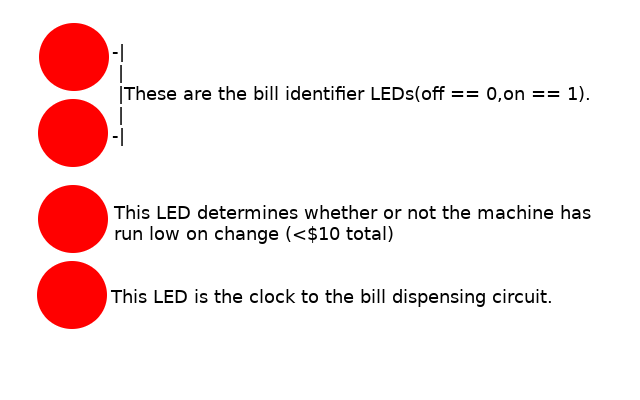
\includegraphics[scale=0.5]{images/LEDs}
\end{itemize}
